% General context + motivation

Neighbourhoods have increasingly become a central concept in social research and
targets for social
policy~\citep{sampson2012great,galster2019making,stone2015urban,looker2015nation}.
To be sure, a focus on neighbourhoods extends to the formative period of the
modern social sciences~\citep{Abbott1997}. Recent interest has at least partly
been rekindled through newly available longitudinal demographic
datasets~\citep{Logan2014,nhgis}, convenient computational
tools~\citep{rey2018spatio}, and new sources of data~\citep{Poorthuis2018}.


\revision{In this work, we consider neighbourhoods as \emph{formal
regions}~\citep{montello2003regions}, geographically continous areas with
similar data characteristics, which these advances made more tractable to
approach in a data-driven fashion.} Yet new challenges have also emerged,
especially at the convergence of research on neighbourhood effects and
neighbourhood dynamics. Neighbourhood effects research assumes knowledge about
the nature and scope of "the neighbourhood" that presumably shapes individual
outcomes~\citep{Kwan2018,Shelton2019}. Concurrently, researchers note that
neighbourhoods are not necessarily fixed containers in which other processes
occur, but themselves dynamically
evolve~\citep{Delmelle2017,Reades2019,li2018new}. The result is to open up key
assumptions about neighbourhoods for theoretical and empirical examination: how
do we appropriately define and compare neighbourhoods at a given time?; how do
we appropriately define and compare the temporal trajectories of
neighbourhoods?; and can we do both at once, "fully
interactionally"~\citep{Abbott1997}: classify neighbourhoods now based on where
they came from and where they are going?


In principle, much of the recent research is committed to the proposition that
neighbourhoods are open and evolving entities. Ironically, its empirical
practice tends to rely on methods that require fixed geographical regions. This
requirement is difficult to satisfy, as most longitudinal datasets are based on
pre-defined tabulation areas that are routinely modified by data collection
agencies, usually to follow population changes. 

The standard approach then is to \emph{geographically harmonise} data. This
involves interpolating existing measurements into a common set of
regions~\citep{Logan2014,Hallisey2017,Allen2018}. Recent computational tools
have somewhat simplified this process~\citep{rey2018spatio}, but it still
involves non-trivial questions: which geometry to use as target, how to
apportion the variables, or how to combine data from different sources. Further,
these question do not necessarily have optimal answers. Indeed, regardless of
how well this process is performed, it still introduces
errors~\citep{Logan2016}, even when additional data is
provided~\citep{eicher2001dasymetric}. Essentially, harmonisation generates
artificial data points that can potentially lead to inaccurate results, even
though they are seldom interpreted as such. Nevertheless, because there has been
no viable alternative, and the results often appear plausible, these concerns
are generally overlooked. The result is that the harmonisation approach is
virtually mandatory in the current literature: \emph{"(...) tract-by-tract
comparison is not possible unless data from 2000 is interpolated to 2010
boundaries (...)"}~\citep{Dmowska2017}, \emph{"(...) This limits cross-year
comparison since data are not representative of the same spatial units. (...)"}
~\citep{Allen2018}. 


The main contribution of this paper is a method for longitudinal data processing
that works with the original data by leveraging a network based representation.
It enables tract-by-tract comparison and the identification of patterns of
demographic evolution \emph{without geographic harmonisation}. 

To allow a proper examination of our method and its results, we built an online
interactive system using this representation. It enables users to visualise,
interpret, and explore trajectories of neighbourhood change. This interface
helps validate our method, by allowing it to be compared to existing and future
methods. Further, it is a significant contribution to the research community: it
provides a vehicle for quickly and easily grasping complex long-term changes,
experimenting with different parameters to interactively learn from data, and
making neighbourhood change research publicly transparent. The interface thus
responds to increasing concerns about reproducibility and transparency, as well
as ongoing attention to the value of visualisation in scientific research and
communication.


We start by presenting an intuitive example of our representation in
Section~\ref{sec:introduction}, then we review the relevant literature on
longitudinal studies, data representation, clustering, and spatio-temporal
visualisation in Section~\ref{sec:related}. Our methodology is introduced in
detail in Section~\ref{sec:method}, along with the included interface.
Illustrative scenarios for Chicago, Toronto, and Los Angeles are presented in
Section~\ref{sec:study} and the feedback of five field experts are summarised in
Section~\ref{sec:expert}. Our prototype system is available at
\censure{\url{http://uoft.me/piccard}}, including more than forty regions in the
US and Canada. The source code is publicly available at
\censure{\url{https://github.com/fabioasdias/piccard}}.\footnote{The editors are
considering, at our request, an exception to the double-blind requirement to
allow access to the system. We provided them with the URLs of the system, code,
and documentation separately.}


\section{Intuition}
\label{sec:intuition}
While utterly simple, the network model breaks from the deeply rooted
traditional tabular paradigm in a significant way. The traditional method
requires the data to be treated as a collection of fixed entities with
properties that evolve over time -- rows in a table with temporal values as
columns. By contrast, our method represents each measurement as a separate
entity and encodes the evolution of these entities over time.

To ease the cognitive transition to a new paradigm, we start with an intuitive
example of how the method works, using a small portion of a fictitious urban
region illustrated on the left part of Figure~\ref{fig:intuition}. This example
includes three different times ($t_0,t_1,t_2$), with different aggregation areas
identified as letters from A to H. For $t_0$, the initial time, we have areas A
and B, with small houses and a park, respectively. The park remains stable (B,
E, and H), but the houses are partially replaced by larger buildings (C and F). 

This example illustrates some of the challenges of harmonisation. None of these
aggregation areas is clearly suitable as an interpolation target. In fact,
adopting any of these areas as a target would require merging heterogeneous
regions and/or dividing homogeneous regions. For instance, by choosing the
regions of $t_1$, A would be split to match regions C and D, which appears to be
a rather reasonable approximation in this homogeneous artificial example (even
if it commits the fallacy of division). Region F would be similarly split to
match C, but F would be split and merged with G to match D, potentially leading
to statistical measurements that do not properly represent either region. 

Real world measurements are seldom as homogeneous and noise-free as this
artificial example. By splitting and merging the data to fit arbitrary borders,
that were not necessarily coherent at the time of the measurement, harmonisation
increases the distance between measurement and reality.


\begin{figure}
    \centering 
    \subfloat{
        \includegraphics[width=0.475\linewidth]{intuition.png}
    }
    \subfloat{
        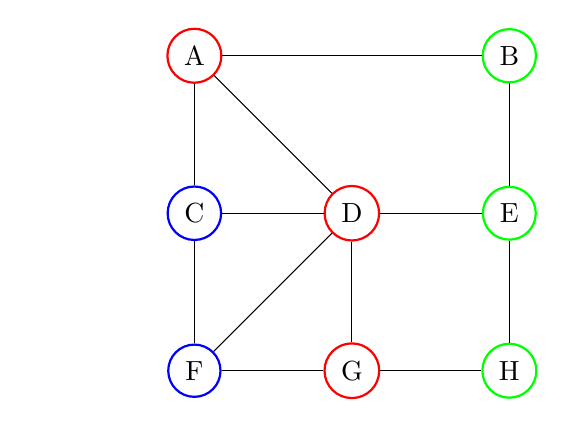
\begin{tikzpicture}
            \node (push) at (-2,0) {};
            \node [circle, draw=red, thick] (a) at (0,4) {A};
            \node [circle, draw=green, thick] (b) at (4,4) {B};
            \node [circle, draw=blue,  thick] (c) at (0,2) {C};
            \node [circle, draw=red, thick] (d) at (2,2) {D};
            \node [circle, draw=green, thick] (e) at (4,2) {E};
            \node [circle, draw=blue, thick] (f) at (0,0) {F};
            \node [circle, draw=red, thick] (g) at (2,0) {G};
            \node [circle, draw=green, thick] (h) at (4,0) {H};
            \draw (a) -- (c);
            \draw (a) -- (b);
            \draw (a) -- (d);
            \draw (b) -- (e);
            \draw (c) -- (f);
            \draw (c) -- (d);
            \draw (d) -- (f);
            \draw (d) -- (e);
            \draw (d) -- (g);
            \draw (e) -- (h);
            \draw (f) -- (g);
            \draw (g) -- (h);
        \end{tikzpicture}
    } \caption{Network based spatio-temporal data representation. \textbf{Left}:
    Three temporal stages of the evolution of a fictitious urban area, with
    aggregation areas A to H. \textbf{Right}: Network representation of the
    aggregation areas where the colours identify similar regions.
        \label{fig:intuition}}
\end{figure}

Instead, we propose a network-based representation. A \emph{network} (also
called a \emph{graph}) is a collection of entities (nodes) that are related to
each other (edges). In this case, each different aggregation area is represented
as a node and we connect nodes that have overlapping geographical areas\revision{ in
different times or are neighbours in the same time}, leading to the network
illustrated on the right of Figure~\ref{fig:intuition}. By partitioning the
network into connected nodes that are similar, we are effectively identifying
clusters in the spatio-temporal data, as illustrated by the colours of the nodes
on the right side of Figure~\ref{fig:intuition}. Further, all the possible paths
of change can be obtained by computing sequences of nodes over time, in this
case: (A, C, F), (A, D, F), (A, D, G), and (B, E, H). This representation is
also suited for geographically consistent regions, as illustrated by the stable
park in this example, and is therefore a generalisation of the traditional
paradigm.

%I'm adding this because Jeff Allen (Farber's guy) struggled with this.
Note that the edges of this network merely encode that two regions are related.
This is binary information, there is no apportionment, no areal measurements,
no population percentages associated with the edge. Indeed, our method also
connects regions of the same time that share borders, representing exactly that
they are neighbouring areas.

In the following, we argue that this network representation allows us to study
neighbourhood change in a way that does not require an prior interpolation. 
